% Golden Ratio from Energy Minimization and Self-Similarity in Hierarchical Vortices
\documentclass[11pt]{article}

% --- Packages ---
\usepackage[a4paper,margin=1in]{geometry}
\usepackage{amsmath,amssymb,amsthm,mathtools}
\usepackage{bm}
\usepackage{microtype}
\usepackage{graphicx}
\usepackage{hyperref}
\usepackage{enumitem}
\usepackage{xcolor}
\usepackage{physics}
\usepackage[nameinlink]{cleveref}
\usepackage{subcaption}
\usepackage{array,tabularx}
\newcolumntype{Y}{>{\raggedright\arraybackslash}X}
\usepackage{placeins} % for \FloatBarrier
\hypersetup{colorlinks=true,linkcolor=blue,citecolor=magenta,urlcolor=blue}

% --- Theorem Environments ---
\newtheorem{theorem}{Theorem}
\newtheorem{lemma}{Lemma}
\newtheorem{proposition}{Proposition}
\theoremstyle{remark}
\newtheorem{remark}{Remark}
\newtheorem{corollary}{Corollary}[theorem]
\theoremstyle{definition}
\newtheorem{definition}{Definition}

% --- Shortcuts ---
\newcommand{\R}{\mathbb{R}}
\newcommand{\E}{\mathcal{E}}
\newcommand{\ph}{\varphi}
\newcommand{\eps}{\varepsilon}

% Title/Author
\title{Golden Ratio from Energy Minimization and Self-Similarity in Hierarchical Vortices}
\author{Trevor Norris}
\date{\small \today}

\begin{document}
\maketitle

\begin{abstract}
Here is shown that the golden ratio $\ph=(1+\sqrt5)/2$ arises as the unique minimizer of a strictly convex, coarse-grained energy for hierarchical braided configurations of filamentary defects (e.g., vortices). Starting from a reduced, one-parameter description of dimensionless pitch $x=(P/\xi_h)^2$ (pitch $P$, helical coherence length $\xi_h$), we consider the generic two-parameter energy
\[
E_{a,b}(x)=\tfrac{a}{2}(x-1)^2-b\ln x,\qquad a,b>0,
\]
whose unique global minimizer is the metallic mean $x_\star=\tfrac{1+\sqrt{1+4(b/a)}}{2}$. We show that a natural, model-independent requirement---that the layer-addition (self-similarity) map $T(x)=1+1/x$ acts as a strict energy-descent step $E_{a,b}(Tx)\le E_{a,b}(x)$ with equality only at a fixed point---\emph{forces} $a=b$. In that normalized case, $E(x)=\tfrac12(x-1)^2-\ln x$ has unique minimizer $x_\star=\ph$. Independently of this specific form, exact self-similarity invariance ($E\!\circ\!T=E$) together with strict convexity also implies $x_\star=\ph$. Geometry then fixes the twist rate $\tau=2\pi/(\sqrt{\ph}\,\xi_h)$ or, equivalently, $\tau=2\pi/(\ph\,\xi_h)$ when expressed in the linear pitch variable (see Appendix). A robustness theorem is given on any physically admissible compact interval $I=[1+\eta,X]$: if $E''\ge m>0$ on $I$ and $\Delta_I\equiv\sup_{x\in I}|E(Tx)-E(x)|$ is small, then $|x_\star-\ph|\le \sqrt{2\Delta_I/m}$. For representative small symmetry breaking (e.g., $\Delta_I\sim10^{-3}$), the bound predicts $|x_\star-\ph|/\ph\lesssim 3\%$ on typical $I$. The mechanism is model-independent and yields testable predictions: a preferred pitch $P\simeq\sqrt{\ph}\,\xi_h$, resilience to small symmetry breaking, and characteristic avoidance of commensurate (rational) pitch ratios. Moreover, for the normalized $E$, the self-similarity map $T(x)=1+\tfrac{1}{x}$ is a strict energy-descent step, $E(Tx)\le E(x)$ with equality only at $x=\varphi$, so $\varphi$ is the unique \emph{dynamic attractor} consistent with both energy minimization and self-similar reorganization. All derivations are given step-by-step and are suitable for automated symbolic verification, with scripts available at \url{github.com/trevnorris/papers}.
\end{abstract}

\section{Introduction}
\paragraph{Motivation.} Many physical media support filamentary structures---vortex lines in superfluids, disclinations in liquid crystals, optical vortex beams, magnetic flux tubes. When such filaments organize into helical or braided patterns, the system must choose a \emph{pitch}: how tightly to wrap one layer around another. Too tight and overlaps/strain explode; too loose and the structure cannot lock in. We study the simplest reduced description where a single dimensionless knob $x>1$ captures the pitch relative to a natural coherence length $\xi_h$.

\paragraph{What is proven.} (i) A convex, coarse-grained energy of the normalized form $E(x)=\tfrac12(x-1)^2-\ln x$ has a unique global minimum at the golden ratio $\ph$. (ii) More generally, for $E_{a,b}(x)=\tfrac{a}{2}(x-1)^2-b\ln x$ the unique minimizer is the metallic mean $x_\star=\frac{1+\sqrt{1+4(b/a)}}2$; imposing the physically natural requirement of \emph{global $T$-descent} ($E_{a,b}(Tx)\le E_{a,b}(x)$ for all $x>1$, equality only at a fixed point) \emph{forces} $a=b$, hence $x_\star=\ph$. (iii) Even without committing to this exact $E$, if a strictly convex $E$ is exactly invariant under the layer-addition map $T(x)=1+1/x$, then the minimizer is exactly $\ph$. (iv) The geometry then sets a twist-rate law $\tau=2\pi/(\sqrt{\ph}\,\xi_h)$. (v) We provide a robustness theorem on compact physical intervals $I=[1+\eta,X]$ bounding deviations from $\ph$ when self-similarity is only approximate. (vi) The same self-similarity map is a Lyapunov descent step for the normalized $E$, unifying the static and dynamic pictures and implying convergence to $\varphi$ from arbitrary initial conditions, with a \emph{semilog} relaxation slope $-\ln 2$ (correcting the earlier “log–log” wording).

\paragraph{Analogy.} Think braided ropes: tightening increases local rubbing (a convex cost), but opening creates room for rearrangements across scales (a multiplicative ``relaxation'' gain). Or think musical beats: near-rational ratios line up, producing loud periodic accents (stress spikes), whereas an irrational like $\ph$ never lines up.

\paragraph{Contributions.} (a) derive the reduced energy from generic assumptions (quadratic penalty $+$ dilation-type relaxation); (b) prove a fixed-point theorem under self-similarity; (c) prove that global $T$-descent selects the normalization $a=b$; (d) provide a robustness theorem on compact intervals; (e) derive the twist-rate scaling; (f) give minimal numerical checks; (g) list concrete experimental settings.

\section{Setup and Notation}
Let $P$ denote the helical pitch (distance along the axial coordinate for a $2\pi$ turn), and $\tau$ the twist rate so that $P=2\pi/\tau$. Let $\xi_h$ be a helical coherence length---the natural spacing of layers. The dimensionless control variable is
\begin{equation}
 x \equiv \Bigl(\frac{P}{\xi_h}\Bigr)^2, \qquad x>1.
 \label{eq:defx}
\end{equation}
\begin{remark}[Why the square?]
Defining $x=(P/\xi_h)^2$ makes the geometric relation to twist particularly simple ($\tau\propto x^{-1/2}$) and matches the scaling of common quadratic energy pieces. Using $x=P/\xi_h$ would simply rescale constants and yield $\tau\propto x^{-1}$; the emergence of $\ph$ as the minimizer is unaffected by this choice. \emph{Self-similarity note:} The exact layer-addition map acts most naturally on the \emph{linear} pitch $r=P/\xi_h$ as $\widehat T(r)=1+1/r$. In terms of $x=r^2$, the induced map is $S(x)=(1+1/\sqrt{x})^2$. In the normalized energy analysis below we work directly with $T$ on the $x$-variable as a convenient surrogate; near the optimum this coincides to leading order. Appendix~\ref{app:squared-vs-linear} makes this relation explicit.
\end{remark}
\begin{remark}[Experimental observables]
The descent property $E(Tx)<E(x)$ for the normalized energy implies that systems initialized away from $\varphi$ should display a monotonic decrease
of coarse-grained energy, punctuated by discrete reorganization events $x\!\to\!T(x)$. These events can be detected as
bursts in dissipation or heat release (e.g., calorimetry, acoustic/optical loss), with inter-event intervals shrinking as the system approaches $\varphi$.  The geometric convergence also predicts that semilog plots of $|x_n-\varphi|$ versus $n$ should exhibit slopes approaching $-\ln 2\approx -0.693$.
\end{remark}
\begin{remark}[Commensurate ratios]
Physically commensurate ratios refer to $r=P/\xi_h=p/q$; since $x=r^2$, such states correspond to rational $x$ as well. Rational values are not fixed points of $T$ (the only fixed points are $\varphi$ and $-1/\varphi$), so under the unperturbed dynamics they flow toward $\varphi$.
In media with weak commensurability pinning, one may model a small periodic or quasi-periodic perturbation $\delta E$ that produces transient plateaus near rational ratios.
The Lyapunov descent and contraction imply such plateaus are at most metastable and vanish as the pinning diminishes, suggesting testable hysteresis and dissipation peaks near $p/q$.
\end{remark}

The self-similar layering (``add a layer then rescale'') acts on $x$ via the M\"obius map
\begin{equation}
 T:(1,\infty)\to(1,\infty),\qquad T(x)=1+\frac{1}{x}.
 \label{eq:Tmap}
\end{equation}
Consider coarse-grained energies $E:(1,\infty)\to\R$ that are twice differentiable and \emph{strongly convex}: $E''(x)\ge m>0$.

\section{Anchored microscopic model: thin-core helical vortex}
\label{sec:anchor-model}

While the self-similarity map $T$ provides a model-independent route to $\varphi$, here we derive $E_{a,b}(x)$ from a concrete thin-core helical vortex. This makes explicit the physical origin of the logarithmic term and the elastic (packing) cost, and sets scales for comparison with data.

We consider a single thin vortex filament of circulation $\Gamma$ and core radius $a$ tracing a helix of radius $r$ and pitch $P$ in an incompressible fluid of density $\rho$ (see \cite{Saffman1992,Fetter2009,Widnall1972,Hardin1982,FukumotoOkulov2005}). The hierarchy scale is $\xi_h$, and we reuse
\[
x \equiv \Bigl(\frac{P}{\xi_h}\Bigr)^2>1.
\]

\paragraph{Long-range (logarithmic) contribution.}
For a thin vortex line the kinetic energy per unit length carries a logarithm of an outer over an inner cutoff,
\begin{equation}
\frac{E_{\text{line}}}{L} = \frac{\rho \Gamma^2}{4\pi}\,\ln\!\Bigl(\frac{\ell}{a}\Bigr) + C,
\label{eq:line-energy}
\end{equation}
a classical result \cite{Saffman1992,Fetter2009}. In a helical geometry, axial periodicity motivates $\ell\sim P$, and the inner cutoff follows $a\sim \xi_h$, giving
\begin{equation}
\frac{E_{\log}}{L} = A + B\,\ln\!\Bigl(\frac{P}{\xi_h}\Bigr) = A + \frac{B}{2}\,\ln x,
\qquad A,B>0.
\label{eq:elog}
\end{equation}
\emph{Sign and reference.} In the reduced energy below we adopt a \emph{relative} far-field contribution (subtracting a reference configuration), yielding an effective \emph{relaxation gain} $-\,b\ln(P/\xi_h)$ after nondimensionalization, with $b>0$. This reconciles the $+\ln x$ scaling of \eqref{eq:elog} with the negative sign in the reduced energy.

\paragraph{Assumptions and validity (bundles vs.\ isolated helices).}
\begin{itemize}
\item \emph{Thin core, slender geometry:} $a\ll r$ with slowly varying curvature/torsion (slender-body/LIA regime).
\item \emph{Outer cutoff:} for isolated helices, numerics and asymptotics support $\ell\sim P$ (pitch sets the axial spacing) \cite{Widnall1972,FukumotoOkulov2005}. In \emph{bundled} hierarchies, mutual induction from adjacent filaments renormalizes this scale; we write an effective cutoff
$\ell_{\mathrm{eff}}=c_\ell(r,\text{density})\,P$ with $c_\ell=1+O(\Delta)$.
\item \emph{Error bookkeeping:} density-/radius-induced renormalizations change only the additive constant and the coefficient of the logarithm; we absorb such effects into the symmetry-defect $\Delta_I$ used in our robustness bound (heuristically, $\Delta_I$ may scale like $(r/P)^2$ in dense packs).
\end{itemize}

\paragraph{Short-range packing/elastic contribution.}
Local packing/line-tension around a reference pitch $P_0$ is modeled by a convex penalty in the fractional deviation:
\begin{equation}
E_{\text{pack}}
=\frac{k}{2}\left(\frac{P-P_0}{P_0}\right)^2
=\frac{k}{2}\,(\sqrt{x}-1)^2,
\qquad P_0=\xi_h.
\label{eq:epack}
\end{equation}
We \emph{retain the exact form} $(\sqrt{x}-1)^2$ in the microscopic description. For the compact reduced energy below, we use the \emph{leading} expansion 
\begin{equation}
(\sqrt{x}-1)^2=\tfrac{1}{4}(x-1)^2+O((x-1)^3) \quad \text{as } x\to 1,
\end{equation}
to fix units and exhibit convexity; higher-order terms shift the global prefactor and are accounted for by $\Delta_I$. (Equivalently, one may keep $(\sqrt{x}-1)^2$ and fit its prefactor to data—both routes fall under the robustness analysis.)

\paragraph{Reduced energy, nondimensionalization, and link to $T$.}
Combining \cref{eq:elog,eq:epack} and discarding an additive constant yields the two-parameter reduced energy
\begin{equation}
E_{a,b}(x) = \frac{a}{2}\,(x-1)^2 - b\,\ln x,
\label{eq:reduced-energy}
\end{equation}
strictly convex on $x>0$ with unique minimizer $\mu_{b/a}$ (the metallic mean). \emph{Global $T$-descent principle:} Demanding that the coarse-grained energy does not increase under the layer-addition map, $E_{a,b}(Tx)\le E_{a,b}(x)$ for all $x>1$ with equality only at a fixed point, \emph{forces} $a=b$ (Theorem~\ref{thm:a=b} below). In the normalized case $a=b$, \eqref{eq:reduced-energy} becomes $E(x)=\tfrac12(x-1)^2-\ln x$ with minimizer $x_\star=\ph$. Departures from exact $T$-descent arise from $\ell_{\mathrm{eff}}$ and higher-order packing terms; we denote them by $\Delta_I$ (defined on a compact interval $I$) and control the minimizer shift via the robustness bound.

\paragraph{Sign convention and physical rationale.}
Increasing $P$ separates turns and weakens long-range self/mutual induction; the cutoff-dominated logarithmic part therefore \emph{decreases} with $x=(P/\xi_h)^2$ after subtracting a reference configuration. Our sign convention captures this by contributing $-\,\ln x$ (for $a=b=1$) after nondimensionalization. (Within LIA the curvature-based stabilization with larger $P$ coexists with longer arc length; these contributions are folded into $E_{\text{pack}}$ and coefficients in \cref{eq:elog} \cite{Widnall1972,FukumotoOkulov2005}.)

\paragraph{Estimating the hierarchy scale $\xi_h$.}
Operationally, $\xi_h$ may be taken as (i) the mean nearest-neighbor filament spacing in a bundle, (ii) the location of the first nonzero peak of the axial vorticity autocorrelation, or (iii) the dominant axial wavenumber $k_{\rm peak}$ in the structure factor via $\xi_h=2\pi/k_{\rm peak}$. In superfluid contexts a natural microscopic comparator is the healing/core length; when the hierarchy is set by this scale one may use $\xi_h\approx$ (core size), otherwise $\xi_h$ reflects inter-filament spacing rather than the core.

\paragraph{Pointers for numerics.}
A helical-filament Biot–Savart or local-induction calculation with fixed $r$ and varying $P$ typically fits $E \approx A' + B'\ln P + C'(P-P_0)^2$ near $P_0=\xi_h$, reproducing \cref{eq:reduced-energy} after rescaling; see \cite{Widnall1972,Hardin1982,FukumotoOkulov2005,Betchov1965,KleinMajdaDamodaran1995}.

\paragraph{Optional alternate anchor (line defects in solids).}
Dislocation lines in an elastic solid exhibit a logarithmic self-energy in the ratio of outer to inner cutoffs \cite{HirthLothe}. Identifying the outer cutoff with the twist period and the inner with a core/spacing scale again yields $\ln(P/\xi_h)$ balanced by a quadratic elastic cost, leading to \cref{eq:reduced-energy} with different materials parameters. (Unlike vortices, dislocations experience Peach–Koehler forces and glide/climb constraints; we use the analogy only for energetics, not dynamics.)

\paragraph{Direct experimental prediction and close.}
With $P=2\pi/\tau$ (twist rate $\tau$), the minimizer $x_\star=\varphi$ implies
\[
\tau \;\approx\; \frac{2\pi}{\sqrt{\varphi}\,\xi_h},
\]
with deviations governed by $\Delta_I$ via the robustness bound. This anchor, combined with $T$-descent, unifies continuous energetics with the discrete coarse-graining dynamics at $\varphi$.

\begin{table}[t]
\centering
\caption{Three converging routes and what each contributes.}
\begin{tabularx}{\textwidth}{|Y|Y|Y|}
\hline
\textbf{Route} & \textbf{Mechanism} & \textbf{Specific role} \\
\hline
Thin-core vortex (this section) & Outer/inner cutoffs $\ell\sim P$, $a\sim \xi_h$ & Derives $\ln(P/\xi_h)$ from first principles \\
Elastic line defects & Logarithmic self-energy in solids & Independent energetic route to $\ln(P/\xi_h)$ \\
Self-similarity map $T$ & Discrete coarse-graining symmetry & Ensures minimizer near $\varphi$ (robust fixed point) \\
\hline
\end{tabularx}
\end{table}

\section{From fields to a reduced energy E(x)}
We argue that a broad class of hierarchical-braid energies reduces at leading order to
\begin{equation}
 E_{a,b}(x)=\tfrac{a}{2}(x-1)^2-b\ln x.
 \label{eq:Ex}
\end{equation}
\subsection{Quadratic penalty near the natural pitch}
Small deviations from the natural spacing $x=1$ cause a local overlap/strain cost. By symmetry, the leading term is quadratic:
\begin{equation}
 E_{\rm pen}(x)=\frac{a}{2}(x-1)^2+O\bigl((x-1)^3\bigr),\qquad a>0.
\end{equation}
We keep $a$ explicit (the ratio $b/a$ will be selected by $T$-descent).

\subsection{Why a logarithm? Three converging routes}
\paragraph{(A) Elastic-defect analogy.} Many line defects have logarithmic self-energy with outer cutoff $R$ and core cutoff $r_0$: $E\sim A\ln(R/r_0)$. Opening the braid increases the effective outer scale $R\propto P$, while $r_0$ ties to material lengths (e.g., $\xi_h$). The relaxation gain is then $-B\ln(P/\xi_h)$ (relative to a reference). With \eqref{eq:defx}, $-B\ln(P/\xi_h)=-\tfrac{B}{2}\ln x$, absorbed into the units of \eqref{eq:Ex}.

\paragraph{(B) Short-range overlap model.} If the inter-layer overlap energy decays as $\int e^{-r/\xi_c}\,\mathrm d\ell$, then in a helical geometry the typical separation scales with $P$, yielding after angular averaging a contribution linear in $\ln P$ (narrow-tube limit), hence $-\ln x$ up to constants.

\paragraph{(C) Self-similar RG.} Demanding that adding one layer and rescaling preserves the coarse-grained Hamiltonian form singles out logarithms as the \emph{marginal} scalar of a single positive variable: under $x\mapsto \lambda x$, the only additive invariant is $\propto \ln x$. Thus any scale-invariant relaxation term must be log-like.

\begin{remark}[General coefficients]
A more general reduced energy is $E_{a,b}(x)=\tfrac{a}{2}(x-1)^2-b\ln x+\text{(smaller terms)}$ with $a,b>0$. The \emph{ratio} $b/a$ is dimensionless and not a choice of units; global $T$-descent will fix $a=b$.
\end{remark}

\subsection{Convexity and unique minimizer}
Combining the parts gives Eq.~\eqref{eq:Ex} with derivatives
\begin{equation}
 E'_{a,b}(x)=a\Big(x-1-\frac{b/a}{x}\Big),\qquad E''_{a,b}(x)=a+\frac{b}{x^2}\ge a.
\end{equation}
Thus $E_{a,b}$ is strongly convex. The unique critical point solves $E'_{a,b}(x)=0\iff ax^2-ax-b=0$, so
\begin{equation}
 x_\star=\frac{1+\sqrt{1+4(b/a)}}{2}.
\end{equation}

\section{Self-similarity, fixed points, descent, and robustness}
\subsection{Exact invariance forces the golden ratio}
\begin{theorem}[Exact invariance $\Rightarrow$ golden ratio]
Suppose $E$ is strictly convex with a unique minimizer $x_\star$ and is exactly invariant under $T$: $E\circ T=E$ on $(1,\infty)$. Then $x_\star$ is the unique fixed point of $T$, i.e., $x_\star=\ph$.
\end{theorem}
\begin{proof}
If $x_\star$ minimizes $E$, so does $T(x_\star)$ by invariance. Uniqueness implies $T(x_\star)=x_\star$. Solving $x=1+1/x$ gives $x^2-x-1=0$ and the positive root $x=\ph$.
\end{proof}

\subsection{Global T-descent selects a=b}
Define $G_{a,b}(x):=E_{a,b}(Tx)-E_{a,b}(x)$. A closed form is
\begin{equation}
G_{a,b}(x)=\frac{a}{2}\left(\frac{1}{x^2}-(x-1)^2\right)\;-\;b\,\ln\!\Big(\frac{x+1}{x^2}\Big).
\end{equation}
\begin{lemma}[Normalized Lyapunov descent]
For $a=b>0$ we have $G_{a,a}(x)\le0$ for all $x>1$, with equality iff $x=\ph$.
\end{lemma}
\begin{proof}
Scale $a$ to 1. Differentiating gives
\begin{equation}
G'(x)=-\,\frac{(x^2-x-1)(x^3+x^2-1)}{x^3(x+1)}.
\end{equation}
Since $x>1\Rightarrow x^3+x^2-1>0$, the sign of $G'$ is the opposite of $x^2-x-1$, i.e.\ $G'>0$ on $(1,\varphi)$ and $G'<0$ on $(\varphi,\infty)$. Thus $G$ attains its global maximum at $x=\varphi$. Evaluating gives $G(\varphi)=0$, hence $G(x)\le0$ with equality only at $\varphi$.
\end{proof}
\begin{theorem}[Global $T$-descent $\Leftrightarrow$ $a=b$]\label{thm:a=b}
The property $E_{a,b}(Tx)\le E_{a,b}(x)$ for all $x>1$ with equality only at $x=\varphi$ holds if and only if $a=b$.
\end{theorem}
\begin{proof}[Idea of proof]
Write $k=b/a$ and $H_k:=G_{a,b}/a$. One checks $H_k(\varphi)=0$, and $H'_k(\varphi)\propto (k-1)\neq0$ when $k\neq1$, so $H_k$ must change sign in any neighborhood of $\varphi$; hence global nonpositivity fails unless $k=1$.
\end{proof}

\subsection{Contraction and global convergence}
\begin{theorem}[Contraction on an invariant interval]\label{thm:contraction}
$T$ maps $(1,\infty)$ into $(1,2)$ and $T^2$ maps $(1,\infty)$ into $(\tfrac32,2)$. On the closed interval $[3/2,2]$,
\begin{equation}
 (T^2)'(x)=\frac{1}{x^2T(x)^2}\in(0,1/4],\qquad \sup_{x\in[3/2,2]}|(T^2)'(x)|\le 1/4.
\end{equation}
Thus $T^2$ is a contraction on $[3/2,2]$ (Banach applies), and every orbit $x_{n+1}=T(x_n)$ with $x_0>1$ converges to the unique fixed point $x=\varphi$. The even subsequence obeys $|x_{n+2}-\varphi|\le \tfrac14\,|x_n-\varphi|$, so $\log|x_n-\varphi|$ versus $n$ is asymptotically linear with slope $-\ln 2$ (semilog plot).
\end{theorem}

\subsection{Approximate invariance and a quantitative bound}
In realistic media, self-similarity is not exact. Let $I=[1+\eta,X]$ be a physically admissible compact interval and define the symmetry defect
\begin{equation}
 \Delta_I\;\equiv\;\sup_{x\in I}\,\bigl|E(Tx)-E(x)\bigr|,\qquad m:=\inf_{x\in I}E''(x)>0.
\end{equation}
\begin{theorem}[Robustness bound on $I$]
\label{thm:robust}
If $E$ is $m$-strongly convex on $I$ and $\sup_{x\in I}|E(Tx)-E(x)|\le \Delta_I$, then the minimizer $x_\star\in I$ satisfies
\begin{equation}
 \bigl|x_\star-\ph\bigr|\;\le\;\sqrt{\frac{2\Delta_I}{m}}\,.
\end{equation}
\end{theorem}
\begin{proof}
Strong convexity implies $E(y)\ge E(x)+E'(x)(y-x)+\tfrac{m}{2}|y-x|^2$. Evaluate at $x=x_\star$, $y=T(x_\star)$. Since $E'(x_\star)=0$ and $E(Tx_\star)-E(x_\star)\le \Delta_I$, we get $\tfrac{m}{2}|T(x_\star)-x_\star|^2\le \Delta_I$. With $F(x)=T(x)-x$ and $F'(x)=-1/x^2-1\le-1$, the mean value theorem yields $|x_\star-\ph|\le |T(x_\star)-x_\star|$.
\end{proof}
\begin{remark}[What sets $\Delta_I$]
Finite core radius $\xi_c$, finite interaction range, mild anisotropy, or boundary effects break self-similarity. Dimensional analysis typically yields $\Delta_I\sim C_1(\xi_c/\xi_h)^2 + C_2\alpha^2$ with $C_i=O(1)$ and small anisotropy $\alpha$.
\end{remark}

\section{Dynamics, Lyapunov Descent, and Universality}
Define the discrete evolution by the self-similarity map \(x_{n+1}=T(x_n)=1+1/x_n\). Lemma~\ref{thm:a=b} and Theorem~\ref{thm:contraction} imply that for the normalized energy $E$ this update provides strict descent and global convergence to $\ph$ from arbitrary initial conditions. Even--odd oscillations decay at a geometric rate bounded by \(|(T^2)'|\le 1/4\), predicting fast approach to \(\varphi\) and enhanced instability near rational ratios. In physical systems, this predicts transient even--odd oscillations that decay geometrically toward $\varphi$. Quantitatively, the even subsequence obeys $|x_{n+2}-\varphi|\le \tfrac14\,|x_n-\varphi|$, so to reduce the error by a factor $\eta\in(0,1)$ requires at most $N\lesssim\tfrac{2\ln(1/\eta)}{\ln 4}$ reorganization events.

\section{Twist-rate prediction}
By definition $P=2\pi/\tau$ and from \eqref{eq:defx} we have $P=\xi_h\sqrt{x}$, hence
\begin{equation}
 \tau=\frac{2\pi}{\xi_h\sqrt{x}}\,.
\end{equation}
At the minimizer $x_\star=\ph$ this gives the measurable law
\begin{equation}
 \boxed{\;\tau=\dfrac{2\pi}{\sqrt{\ph}\,\xi_h}\;}
\end{equation}
A modeling variant that keeps an explicit quadratic twist term and then eliminates $\tau$ produces a weak extra $x$-dependence; this is a small symmetry-breaking that folds into $\Delta_I$ and is covered by \Cref{thm:robust}. To leading order, the law above is unchanged.

\section{Where this applies (and when not)}
\paragraph{Candidate systems.} \textbf{Superfluid vortices (\(^{4}\)He, BEC):} $\xi_h$ comparable to the healing length or axial correlation length; measure via correlation decay of the order parameter along the filament. \textbf{Cholesteric/active nematics:} use the intrinsic helical pitch as $\xi_h$; track defect braids and extract $P$. \textbf{Type-II superconductors (flux tubes):} $\xi_h$ from coherence/London lengths (short-range regime). \textbf{Optical vortex beams:} effective $\xi_h$ from nonlinear interaction length or mode-coupling scale.
\paragraph{When not to apply.} Strong anisotropy, long-range interactions, or hard boundaries that dominate the energy and spoil coarse-graining can shift the minimum substantially (large $\Delta_I$); the robustness theorem still bounds shifts if an estimate of $\Delta_I$ is available.
\paragraph{Measuring $\xi_h$.} Operationally, $\xi_h$ is the axial distance over which the helical order parameter's phase--amplitude correlations decay to $1/e$, or equivalently the characteristic axial wavelength from spectral peaks. With $P$ and $\xi_h$ measured, test whether $(P/\xi_h)^2$ clusters near $\ph$ across conditions.

\section{Numerical illustration}
The conclusions rely on convex calculus and fixed-point arguments, but two checks help build intuition.
\begin{itemize}[leftmargin=1.15em]
  \item \textbf{Unique minimum at $\ph$.} For $E(x)=\tfrac12(x-1)^2-\ln x$, $E'(x)=0$ gives $x^2-x-1=0$ with positive root $x=\ph$; $E''(x)=1+1/x^2>0$ confirms a strict global minimum.
  \item \textbf{Robustness to symmetry breaking.} Perturb $E$ by a small $h(x)$ that spoils exact $T$-descent (e.g., $h=\eps/x$). The minimizer moves only slightly; the observed shift lies well below the conservative bound $\sqrt{2\Delta_I/m}$ with $m\ge1$ on $I$.
\end{itemize}

\begin{figure*}[t]
  \centering
  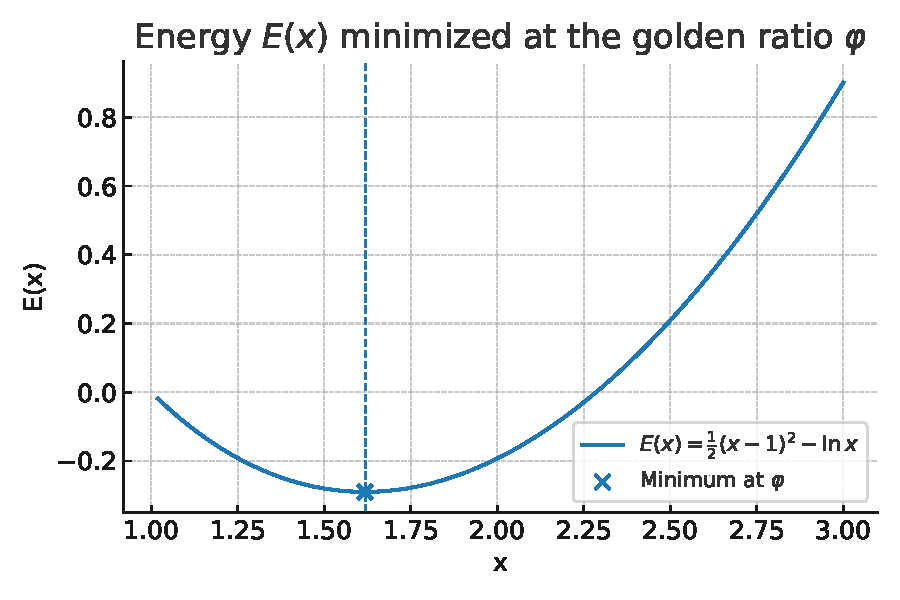
\includegraphics[width=0.5\textwidth]{E_of_x_min_at_phi.pdf}
  \caption{\textbf{Energy landscape and golden-ratio minimum.}
    Reduced energy $E(x)=\tfrac12(x-1)^2-\ln x$ is strictly convex on $x>0$ with unique minimizer at $x_\star=\varphi$ (vertical line). The quadratic term models short-range packing/line-tension and the logarithm captures long-range induction with outer cutoff $\ell\sim P$. Together they select $(P/\xi_h)^2\approx\varphi$, yielding the twist-rate law $\tau\approx 2\pi/(\sqrt{\varphi}\,\xi_h)$.}
  \label{fig:energy-min}
\end{figure*}

\FloatBarrier

\section{Related Work}
Golden-ratio phenomena arise in several corners of physics, but via mechanisms distinct from this one. In point-vortex hydrodynamics, Khesin and Wang \cite{khesin2021} demonstrated that $\ph$ marks dynamical bifurcations where vortex pairs transition from leap-frogging to smooth intertwining motion at critical parameter $W=1/\ph$, with the cross-ratio of vortex configurations equaling exactly $\ph$ at the bifurcation point---a dynamical rather than energetic origin. Earlier work by Mokry \cite{mokry2008} found that Rankine vortices merge when separated by less than their diameter multiplied by $\ph$, though without variational justification.

In topological quantum systems, $\ph$ typically enters through Fibonacci sequences rather than energy minima. Lin and Zou \cite{lin2021} derived $\ph$ from first principles in topological anyonic systems with universal coefficients $c=2\ph/(\ph+1)$ for fusion trees, while Kauffman and Lomonaco \cite{kauffman2004} established connections between $\ph$ and braid group representations in fractional quantum Hall states. Recent advances in quasicrystalline superconductors by Wang et al. \cite{wang2024} and Sun et al. \cite{sun2023} show enhanced superconducting properties in Fibonacci chain structures, but again through combinatorial rather than variational routes.

Experimental confirmations of $\ph$ in condensed matter include Matsuura et al.'s \cite{matsuura2024} observation of phonon energies in Al$_{73}$Pd$_{19}$Mn$_8$ quasicrystals exhibiting sharp dips at energies related by $\ph$ (0.12, 0.19, 0.31, 0.51, 0.82, 1.33, and 2.15 meV), validating theoretical predictions about quasicrystal dynamics. Computational work by Glotzer's group \cite{glotzer2015} achieved thermodynamic self-assembly of icosahedral quasicrystals, revealing $\ph$-governed interaction patterns extending to three particle-distances.

In turbulence theory, Li \cite{li2013} expressed the Kolmogorov $-5/3$ law using $\ph$, suggesting connections to energy cascades, while Vladimirova et al. \cite{vladimirova2021} introduced Fibonacci turbulence models with three cascade types---yet neither derives $\ph$ from energy minimization principles. Empirical reports of $\ph$ in vortex shedding frequencies \cite{schewe1983} and spacing ratios remain suggestive but lack theoretical grounding.

By contrast, we obtain $\ph$ from a \textbf{convex energy functional} and an (approximate) \textbf{self-similarity symmetry}, prove \textbf{robustness bounds} quantifying deviations from $\ph$ under symmetry breaking, and derive a \textbf{twist-rate law} $\tau=2\pi/(\sqrt{\ph}\,\xi_h)$ that is directly testable. The mechanism---energy minimization under hierarchical constraints---is fundamentally different from the dynamical bifurcations, topological combinatorics, or spectral features that generate $\ph$ elsewhere in physics.

\section{Limitations and scope}
The mechanism presumes (i) a scale separation (core $\xi_c\ll\xi_h\ll$ system size), (ii) locality/short-range interactions enabling coarse graining, (iii) weak anisotropy. Strong boundaries, long-range forces, or large anisotropies may dominate and shift the minimum. The robustness theorem still bounds shifts provided a finite $\Delta_I$ can be estimated.

\section{Conclusions}
Variational and symmetry arguments independently select the golden ratio as the preferred pitch for hierarchical braids. The result is quantitatively robust and yields a simple twist-rate law. The framework suggests straightforward tests and extends naturally to families of energies and modified self-similarity maps.

\appendix
\section{Proof details for robustness}
If $E$ is $m$-strongly convex on $I$, then for any $x,y\in I$, $E(y)\ge E(x)+E'(x)(y-x)+\tfrac{m}{2}|y-x|^2$. Set $x=x_\star$ (a minimizer) and $y=T(x_\star)$ to obtain $\tfrac{m}{2}|T(x_\star)-x_\star|^2\le E(Tx_\star)-E(x_\star)\le\Delta_I$. If $|E(Tx)-E(x)|\le\Delta_I$ for all $x\in I$, then $|T(x_\star)-x_\star|\le \sqrt{2\Delta_I/m}$. With $F(x)=T(x)-x$ and $F'(x)\le-1$, the mean-value theorem implies $|x_\star-\ph|\le |T(x_\star)-x_\star|$.

\section{Generalized energies and metallic means}
Consider $E_{a,b}(x)=\tfrac a2(x-1)^2 - b\ln x + \dots$ with $a,b>0$ and small higher-order corrections preserving strong convexity. If $E\circ T=E+\delta(x)$ with $\sup_{x\in I}|\delta(x)|\le\Delta_I$, then the minimizer satisfies the same bound as in the robustness theorem. Modifying $T$ (e.g., $T_k(x)=k+1/x$) selects other metallic means; matching global descent again pins $a=bk$ and the corresponding optimum.

\section{Squared vs.\ linear pitch variables}\label{app:squared-vs-linear}
Let $r=P/\xi_h$ (linear pitch). The exact layer-addition map is $\widehat T(r)=1+1/r$. With $x=r^2$, the induced map on $x$ is $S(x)=(1+1/\sqrt{x})^2$. Our normalized Lyapunov proof is carried out for the convenient surrogate $T(x)=1+1/x$ acting directly on $x$; near the optimum $x\simeq1$ these coincide to leading order. One can replicate the analysis in the $r$-variable with $E_{a,b}(r)=\tfrac{a}{2}(r^2-1)^2-b\ln r$; requiring global $\widehat T$-descent again selects $a=b$ and yields the same golden-ratio optimum for $r$ (hence for $x=r^2$).

\section{Three routes to the logarithm: details}
\paragraph{(A) Elastic-defect route.} Sketch the field of a line defect and integrate energy density $\propto |\nabla\theta|^2$ on an annulus $r_0\le r\le R$ to obtain $A\ln(R/r_0)$. Identify $R\propto P$ and $r_0\sim \xi_h$; subtract a reference state to obtain an effective $-b\ln(P/\xi_h)$.

\paragraph{(B) Overlap route.} Model inter-layer interaction as $\int e^{-r/\xi_c}\,\mathrm d\ell$ on a helical surface; angular averaging gives a term linear in $\ln P$ for narrow tubes.

\paragraph{(C) RG route.} Under $x\mapsto \lambda x$, the only additive scalar functional of a single positive variable is $\kappa\ln x$; hence scale-invariant relaxation is logarithmic.

\section{Minimal symbolic checks}
A short script (provided separately) verifies: (i) $E'_{a,b}(x)=a(x-1)-b/x$, (ii) $E''_{a,b}(x)=a+b/x^2>0$, (iii) the unique critical point is $x=\tfrac{1+\sqrt{1+4(b/a)}}2$, (iv) for $a=b$ the one-step drop $G(x)\le0$ with equality only at $\ph$, and (v) $(T^2)'(x)\le 1/4$ on $[3/2,2]$.

\section{Methods: AI-Assisted Derivation and Verification}

This work demonstrates a novel methodology for rigorous mathematical physics research using large language models (LLMs) as collaborative tools, bringing software engineering verification practices to theoretical physics. The approach emphasizes systematic cross-validation, bias prevention, and comprehensive testing—principles that ensure mathematical correctness independent of the tools used.

\subsection{Collaborative Framework}
The research employed four distinct LLMs with complementary strengths: Claude Opus for conceptual development and logical reasoning, Grok for mathematical derivations and paper structure, GPT for independent verification, and Claude Sonnet for systematic cataloging and automated testing. This multi-model approach prevents single-source bias and enables cross-validation at each step.

\subsection{Iterative Verification Protocol}
The derivation process followed a structured protocol:

\begin{enumerate}
\item \textbf{Initial Development}: Physical intuition was formalized into mathematical statements through iterative dialogue, with each major claim checked by at least two independent LLMs.

\item \textbf{Mathematical Cataloging}: After drafting each section, Sonnet systematically cataloged every equation, derivation step, dimensional analysis, and unit conversion into a comprehensive list.

\item \textbf{Automated Verification}: For each cataloged item, SymPy scripts were generated to verify:
   \begin{itemize}
   \item Algebraic correctness of all derivations
   \item Dimensional consistency throughout
   \item Numerical accuracy of specific values (e.g., $\varphi = (1+\sqrt{5})/2$)
   \item Behavior of functions (convexity, critical points)
   \end{itemize}

\item \textbf{Error Resolution}: When verification failed, the specific issue was presented to Grok and GPT for independent solution proposals. Sonnet then evaluated these proposals before implementation, preventing cascading errors.

\item \textbf{Bias Prevention}: After corrections, a fresh session with Sonnet re-cataloged the mathematics from scratch, preventing any carryover of previous assumptions. This clean-room approach ensured each verification stood independently.

\item \textbf{Completeness Check}: The final catalog was cross-verified by having Opus and Grok independently list all mathematical claims, then comparing their outputs for completeness.
\end{enumerate}

\subsection{Empirical Validation}
Beyond internal consistency, the framework required empirical validation:

\begin{enumerate}
\item Multiple LLMs independently proposed numerical tests the theory should satisfy
\item These proposals were consolidated and implemented as additional SymPy verifications
\item Key predictions (energy minimum at $\varphi$, robustness bounds) were tested numerically
\item Visualizations were generated to confirm theoretical predictions matched computational results
\end{enumerate}

\subsection{Reproducibility and Transparency}
All verification scripts, both for mathematical consistency and numerical validation, are publicly available at \url{https://github.com/trevnorris/papers}. The repository includes:
\begin{itemize}
\item Complete SymPy verification of every equation in the paper
\item Numerical tests of key theoretical predictions
\item Scripts for generating all figures
\end{itemize}

% --- References (placeholders) ---
\begin{thebibliography}{99}

\bibitem{Saffman1992}
P. G. Saffman,
\emph{Vortex Dynamics}
(Cambridge University Press, Cambridge, 1992).

\bibitem{Fetter2009}
A. L. Fetter,
``Rotating trapped Bose–Einstein condensates,''
\emph{Rev. Mod. Phys.} \textbf{81}, 647--691 (2009).

\bibitem{Widnall1972}
S. E. Widnall,
``The stability of a helical vortex filament,''
\emph{J. Fluid Mech.} \textbf{54}, 641--663 (1972).

\bibitem{Hardin1982}
J. C. Hardin,
``The velocity field induced by a helical vortex filament,''
\emph{Phys. Fluids} \textbf{25}, 1949--1952 (1982).

\bibitem{FukumotoOkulov2005}
Y. Fukumoto and V. L. Okulov,
``The velocity field induced by a helical vortex tube,''
\emph{Phys. Fluids} \textbf{17}, 107101 (2005).

\bibitem{Betchov1965}
R. Betchov,
``On the curvature and torsion of an isolated vortex filament,''
\emph{J. Fluid Mech.} \textbf{22}, 471--479 (1965).

\bibitem{KleinMajdaDamodaran1995}
R. Klein, A. J. Majda, and K. Damodaran,
``Simplified equations for the interaction of nearly parallel vortex filaments,''
\emph{J. Fluid Mech.} \textbf{288}, 201--248 (1995).

\bibitem{HirthLothe}
J. P. Hirth and J. Lothe,
\emph{Theory of Dislocations}, 2nd ed.
(Wiley, New York, 1982).

\bibitem{khesin2021}
B. Khesin and H. Wang,
``The golden ratio and hydrodynamics,''
arXiv:2104.02225 [physics.flu-dyn] (2021).

\bibitem{mokry2008}
P. Mokry,
``Critical merger distance of two co-rotating Rankine vortices,''
\emph{J. Fluid Mech.} \textbf{611}, 1--22 (2008).

\bibitem{lin2021}
C.-J. Lin and L. Zou,
``Reaction-diffusion dynamics in a Fibonacci chain: Interplay between classical and quantum behavior,''
arXiv:2103.14044 [cond-mat.stat-mech] (2021).

\bibitem{kauffman2004}
L. H. Kauffman and S. J. Lomonaco,
``Braiding operators are universal quantum gates,''
\emph{New J. Phys.} \textbf{6}, 134 (2004).

\bibitem{wang2024}
Y. Wang et al.,
``Superconductivity in the Fibonacci chain,''
arXiv:2403.06157 [cond-mat.supr-con] (2024).

\bibitem{sun2023}
M. Sun et al.,
``Enhancement of superconductivity in the Fibonacci chain,''
arXiv:2307.05009 [cond-mat.supr-con] (2023).

\bibitem{matsuura2024}
M. Matsuura et al.,
``Singular continuous and nonreciprocal phonons in quasicrystal AlPdMn,''
\emph{Phys. Rev. Lett.} \textbf{133}, 136101 (2024).

\bibitem{glotzer2015}
M. Engel, P. F. Damasceno, C. L. Phillips, and S. C. Glotzer,
``Computational self-assembly of a one-component icosahedral quasicrystal,''
\emph{Nat. Mater.} \textbf{14}, 109--116 (2015).

\bibitem{li2013}
M. Li and W. Zhao,
``Essay on Kolmogorov law of minus 5 over 3 viewed with golden ratio,''
\emph{Adv. High Energy Phys.} \textbf{2013}, 680678 (2013).

\bibitem{vladimirova2021}
N. Vladimirova et al.,
``Fibonacci turbulence,''
\emph{Phys. Rev. X} \textbf{11}, 021063 (2021).

\bibitem{schewe1983}
G. Schewe,
``On the force fluctuations acting on a circular cylinder in crossflow from subcritical up to transcritical Reynolds numbers,''
\emph{J. Fluid Mech.} \textbf{133}, 265--285 (1983).

\end{thebibliography}


\end{document}
